\chapter{Image classification}


\section{Supervised datasets}

\begin{description}
    \item[Dataset] \marginnote{Dataset}
        Given a set of labeled data, it can be split into:
        \begin{descriptionlist}
            \item[Train set] $D^\text{train} = \{ (\text{x}_\text{train}^{(i)}, y_\text{train}^{(i)}) \mid i = 1, \dots, N \}$.
            \item[Test set] $D^\text{test} = \{ (\text{x}_\text{test}^{(i)}, y_\text{test}^{(i)}) \mid i = 1, \dots, M \}$.
        \end{descriptionlist}

        It is assumed that the two sets contain i.i.d. samples drawn from the same unknown distribution.
\end{description}


\subsection{Modified NIST (MNIST)}

\begin{minipage}{0.45\linewidth}
    \centering
    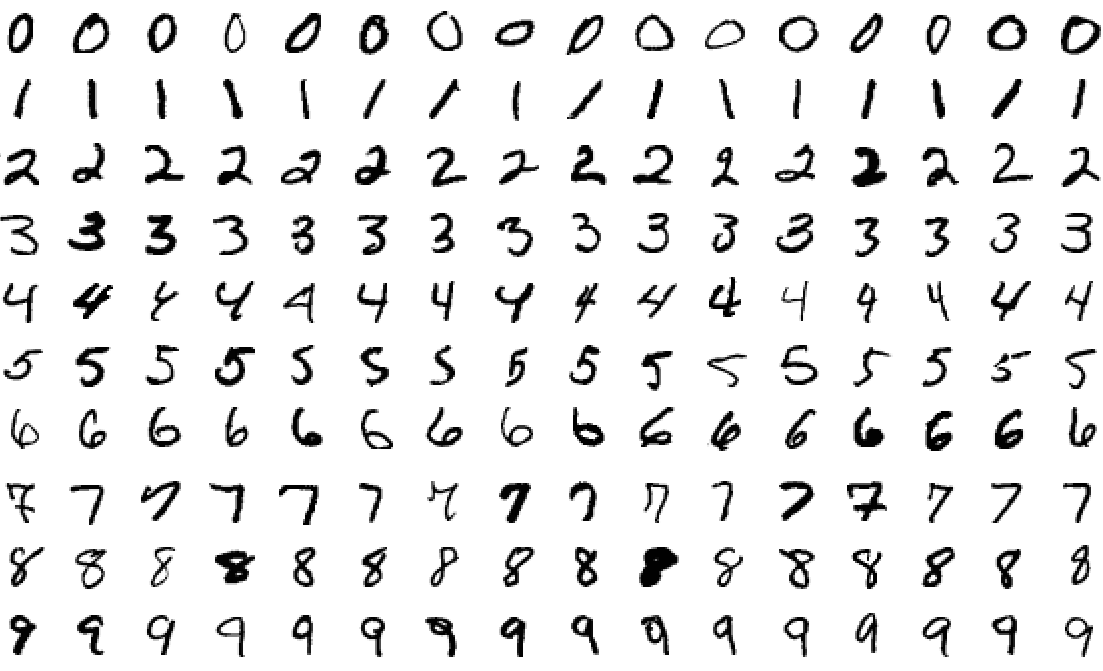
\includegraphics[width=0.9\linewidth]{./img/mnist.png}
\end{minipage}
\begin{minipage}{0.5\linewidth}
    \begin{descriptionlist}
        \item[Content] Handwritten digits from 0 to 9.
        \item[Number of classes] 10.
        \item[Train set size] 50k.
        \item[Test set size] 10k.
        \item[Image format] $28 \times 28$ grayscale.
    \end{descriptionlist}
\end{minipage}


\subsection{CIFAR10}

\begin{minipage}{0.45\linewidth}
    \centering
    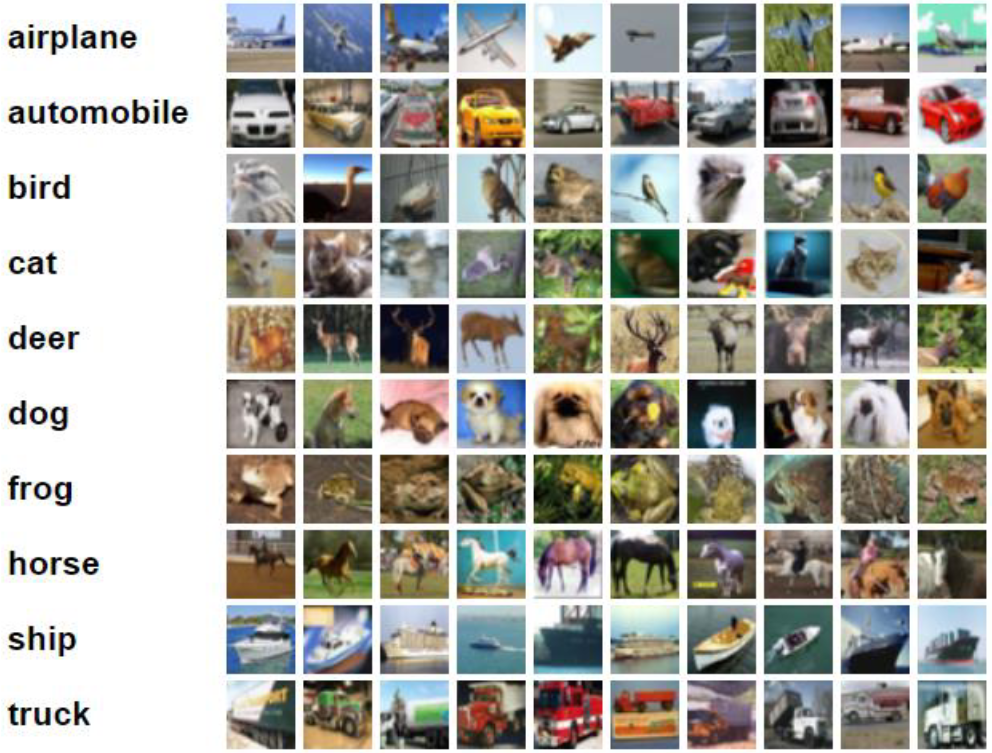
\includegraphics[width=0.9\linewidth]{./img/cifar10.png}
\end{minipage}
\begin{minipage}{0.5\linewidth}
    \begin{descriptionlist}
        \item[Content] Objects of various categories.
        \item[Number of classes] 10.
        \item[Train set size] 50k.
        \item[Test set size] 10k.
        \item[Image size] $32 \times 32$ RGB.
    \end{descriptionlist}
\end{minipage}


\subsection{CIFAR100}

\begin{minipage}{0.45\linewidth}
    \centering
    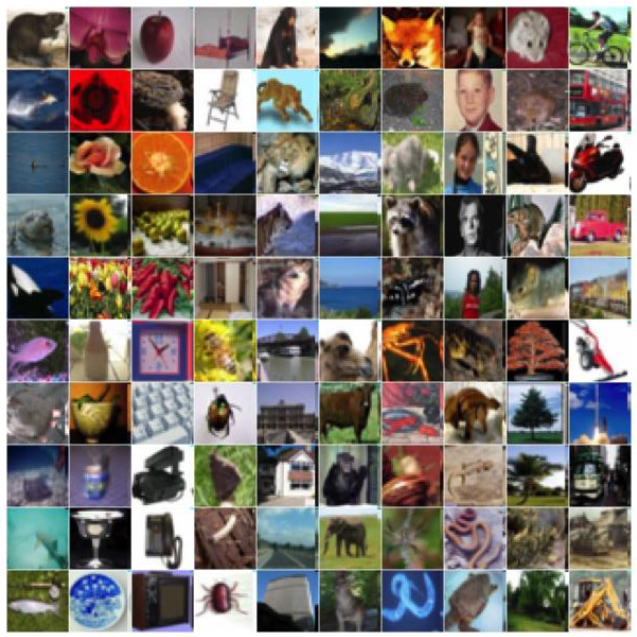
\includegraphics[width=0.7\linewidth]{./img/cifar100.png}
\end{minipage}
\begin{minipage}{0.5\linewidth}
    \begin{descriptionlist}
        \item[Content] Objects of various categories.
        \item[Number of classes] 100 (20 super-classed with 5 sub-classes).
        \item[Train set size] 50k.
        \item[Test set size] 10k.
        \item[Image size] $32 \times 32$ RGB.
    \end{descriptionlist}
\end{minipage}


\subsection{ImageNet 21k}

\begin{descriptionlist}
    \item[Content] Objects of various categories.
    \item[Number of classes] 21k synsets from WordNet organized hierarchically.
    \item[Dataset size] 14 millions.
    \item[Image size] Variable resolution RGB. Average size of $400 \times 350$.
\end{descriptionlist}

\begin{figure}[H]
    \centering
    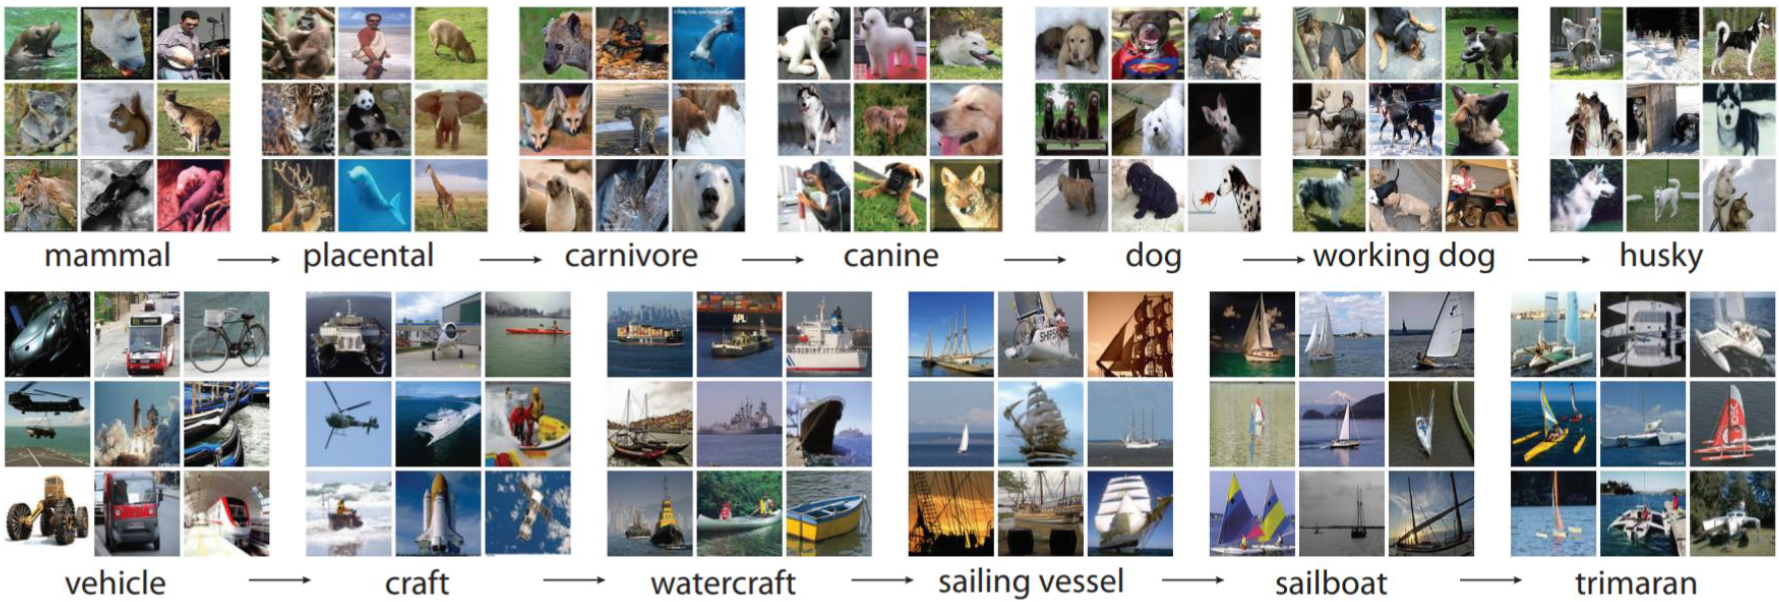
\includegraphics[width=0.85\linewidth]{./img/imagenet21k.png}
\end{figure}


\subsection{ImageNet 1k}

\begin{minipage}{0.45\linewidth}
    \centering
    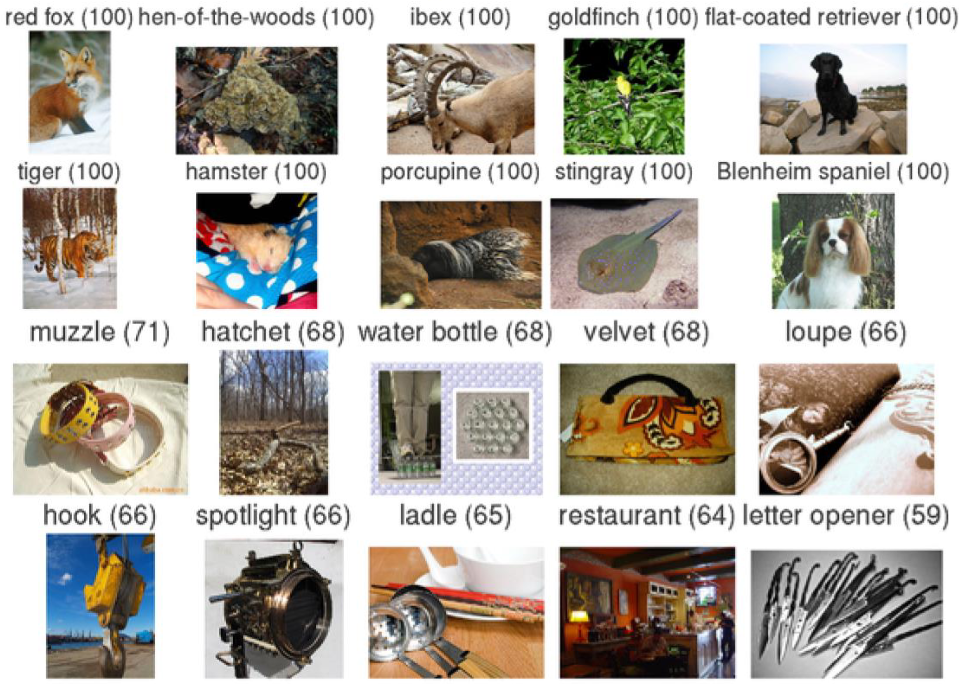
\includegraphics[width=\linewidth]{./img/imagenet1k.png}
\end{minipage}
\begin{minipage}{0.5\linewidth}
    \begin{descriptionlist}
        \item[Content] Objects of various categories.
        \item[Number of classes] 1000.
        \item[Train set size] $1.3$ millions.
        \item[Validation set size] 50k.
        \item[Test set size] 100k.
        \item[Image size] Variable resolution RGB. Often resized to $256 \times 256$.
    \end{descriptionlist}
\end{minipage}

\begin{remark}
    Performance is usually measured as top-5 accuracy as making a single prediction might be ambiguous due to the fact that the images can contain multiple objects.
\end{remark}



\section{Learning}

\begin{description}
    \item[Learning problem] \marginnote{Learning problem}
        Find the best model $h^*$ from the hypothesis space $\mathbb{H}$ that minimizes a loss function $\mathcal{L}$:
        \[ h^* = \arg\min_{h \in \mathbb{H}} \mathcal{L}(h, \matr{D}^\text{train}) \]

        In machine learning, models are usually parametrized. The problem then becomes to find the best set of parameters $\matr{\theta}^*$ from the parameter space $\Theta$:
        \[ \matr{\matr{\theta}}^* = \arg\min_{\matr{\theta} \in \Theta} \mathcal{L}(\matr{\theta}, \matr{D}^\text{train}) \]
\end{description}


\subsection{Loss function}

\begin{description}
    \item[Loss function] \marginnote{Loss function}
        Easy to optimize function that acts as a proxy to measure the goodness of a model.

        The loss computed on a dataset is usually obtained as the average of the values of the single samples:
        \[ \mathcal{L}(\matr{\theta}, \matr{D}^\text{train}) = \frac{1}{N} \sum_{i}^{\vert \matr{D}^\text{train} \vert} \mathcal{L}\big( \matr{\theta}, (\vec{x}^{(i)}, y^{(i)}) \big) \]


    \item[0-1 loss] \marginnote{0-1 loss}
        Loss computed as the number of misclassifications:
        \[ \mathcal{L}\big( \matr{\theta}, (\vec{x}^{(i)}, y^{(i)}) \big) = \vert \text{misclassifications} \vert \]

        This loss is not ideal as it is insensitive to small (or even large) changes in the parameters.
        Moreover, it does not tell in which direction should the parameters be modified to reduce the loss.

        \begin{remark}
            This loss can be minimized using a combinatorial optimization approach but it does not scale well with large datasets.
        \end{remark}

        \begin{figure}[H]
            \centering
            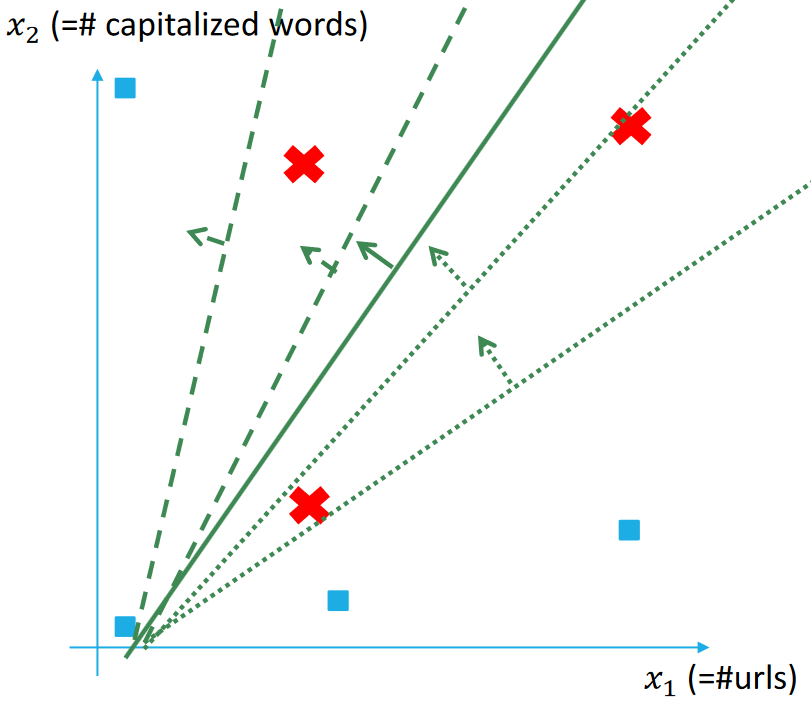
\includegraphics[width=0.3\linewidth]{./img/01_loss_spam.png}
            \caption{\parbox[t]{0.7\linewidth}{
                    Example of linear classifier for spam detection. 
                    Small changes on the boundary line do not change the 0-1 loss. 
                    The loss itself does not tell which is the best direction to move the line.
            }}
        \end{figure}


    \item[Root mean square error] \marginnote{Root mean square error}
        Loss computed as the direct comparison between the prediction and target label:
        \[ \mathcal{L}\big( \matr{\theta}, (\vec{x}^{(i)}, y^{(i)}) \big) = \Vert f(\vec{x}^{(i)}; \matr{\theta}) - y^{(i)} \Vert_2 \]
        Note that $y^{(i)}$ might be encoded (e.g. one-hot).


    \item[Cross-entropy loss] \marginnote{Cross-entropy loss}
        Transform the logits of a model into a probability distribution and estimate the parameters through MLE.

        \begin{descriptionlist}
            \item[Softmax] \marginnote{Softmax}
                Function that converts its input into a probability distribution.
                Given the logits $\vec{s} \in \mathbb{R}^{c}$, the score $\vec{s}_j$ of class $j$ is converted into a probability as follows:
                \[ 
                    \mathcal{P}_\text{model}(Y = j | X = \vec{x}^{(i)}; \matr{\theta}) = 
                        \texttt{softmax}_j(\vec{s}) = 
                        \frac{\exp(\vec{s}_j)}{\sum_{k=1}^{c} \exp(\vec{s}_k)} 
                \]

                For numerical stability, \texttt{softmax} is usually computed as:
                \[
                    \begin{split}
                        \texttt{softmax}_j(\vec{s} - \max\{ \vec{s} \}) &= \frac{\exp(\vec{s}_j - \max\{ \vec{s} \})}{\sum_{k=1}^{c} \exp(\vec{s}_k - \max\{ \vec{s} \})} \\
                        &= \frac{\cancel{\exp(- \max\{ \vec{s} \})}\exp(\vec{s}_j)}{\cancel{\exp(- \max\{ \vec{s} \})}\sum_{k=1}^{c} \exp(\vec{s}_k)} = \texttt{softmax}_j(\vec{s})
                    \end{split}    
                \]
            
            \item[Maximum likelihood estimation] \marginnote{Cross-entropy loss}
                Use MLE to estimate the parameters on the probability distribution outputted by the \texttt{softmax} function:
                \[
                    \begin{split}
                        \matr{\theta}^* &= \arg\max_\matr{\theta} \mathcal{P}_\text{model}(y^{(1)}, \dots, y^{(N)} | \vec{x}^{(1)}, \dots, \vec{x}^{(N)}; \matr{\theta}) \\
                            &= \arg\max_\matr{\theta} \prod_{i=1}^{N} \mathcal{P}_\text{model}(Y = y^{(i)} | X=\vec{x}^{(i)}; \matr{\theta}) \\
                            &= \arg\max_\matr{\theta} \sum_{i=1}^{N} \log\mathcal{P}_\text{model}(Y = y^{(i)} | X=\vec{x}^{(i)}; \matr{\theta}) \\
                            &= \arg\min_\matr{\theta} \sum_{i=1}^{N} -\log\mathcal{P}_\text{model}(Y = y^{(i)} | X=\vec{x}^{(i)}; \matr{\theta}) \\
                            &= \arg\min_\matr{\theta} \sum_{i=1}^{N} -\log\left( \frac{\exp(\vec{s}_{y^{(i)}})}{\sum_{k=1}^{c} \exp(\vec{s}_k)} \right) \\
                            &= \arg\min_\matr{\theta} \sum_{i=1}^{N} -\log\left( \exp(\vec{s}_{y^{(i)}}) \right) + \log\left( \sum_{k=1}^{c} \exp(\vec{s}_k) \right) \\
                            &= \arg\min_\matr{\theta} \sum_{i=1}^{N} -\vec{s}_{y^{(i)}} + \log\left( \sum_{k=1}^{c} \exp(\vec{s}_k) \right) \\
                    \end{split}    
                \]

                The second term ($\log\left( \sum_{k=1}^{c} \exp(\vec{s}_k)\right)$) is called \texttt{logsumexp} and approximates the max function.
                Therefore, the loss can be seen as:
                \[ 
                    \mathcal{L}\big( \matr{\theta}, (\vec{x}^{(i)}, y^{(i)}) \big) 
                    = -\vec{s}_{y^{(i)}} + \log\left( \sum_{k=1}^{c} \exp(\vec{s}_k) \right) 
                    \approx -\vec{s}_{y^{(i)}} + \max\{ \vec{s} \}
                \]
        \end{descriptionlist}
        
\end{description}


\subsection{Gradient descent}

\begin{description}
    \item[Gradient descent] \marginnote{Gradient descent}
        An epoch $e$ of gradient descent does the following:
        \begin{enumerate}
            \item Classify all training data to obtain the predictions $\hat{y}^{(i)} = f(\vec{x}^{(i)}; \matr{\theta}^{(e-1)})$
                and the loss $\mathcal{L}(\matr{\theta}^{(e-1)}, \matr{D}^\text{train})$.
            \item Compute the gradient $\nabla \mathcal{L} = \frac{\partial\mathcal{L}}{\partial \matr{\theta}} (\matr{\theta}^{(e-1)}, \matr{D}^\text{train})$.
            \item Update the parameters $\matr{\theta}^{(e)} = \matr{\theta}^{(e-1)} - \texttt{lr} \cdot \nabla \mathcal{L}$.
        \end{enumerate}

    \item[Stochastic gradient descent] \marginnote{Stochastic gradient descent}
        Reduce the computational cost of gradient descent by computing the gradient of a single sample.
        An epoch $e$ of SGD does the following:
        \begin{enumerate}
            \item Shuffle the training data $\matr{D}^\text{train}$.
            \item For $i = 0, \dots, N-1$:
            \begin{enumerate}
                \item Classify $\vec{x}^{(i)}$ to obtain the prediction $\hat{y}^{(i)} = f(\vec{x}^{(i)}; \matr{\theta}^{(e*N+i)})$
                and the loss $\mathcal{L}\big( \matr{\theta}^{(e*N+i)}, (\vec{x}^{(i)}, y^{(i)}) \big)$.
                \item Compute the gradient $\nabla \mathcal{L} = \frac{\partial\mathcal{L}}{\partial \matr{\theta}}\big( \matr{\theta}^{(e*N+i)}, (\vec{x}^{(i)}, y^{(i)}) \big)$.
                \item Update the parameters $\matr{\theta}^{(e*N+i+1)} = \matr{\theta}^{(e*N+i)} - \texttt{lr} \cdot \nabla \mathcal{L}$.
            \end{enumerate}
        \end{enumerate}

    \item[SGD with mini-batches] \marginnote{SGD with mini-batches}
        Increase the update accuracy of SGD by using a mini-batch.
        An epoch $e$ of SGD with mini-batches of size $B$ does the following:
        \begin{enumerate}
            \item Shuffle the training data $\matr{D}^\text{train}$.
            \item For $u = 0, \dots, U$, with $U = \lceil \frac{N}{B} \rceil$:
            \begin{enumerate}
                \item Classify the examples $\matr{X}^{(u)} = \{ \vec{x}^{(Bu)}, \dots, \vec{x}^{(B(u+1)-1)} \}$ 
                    to obtain the predictions $\hat{Y}^{(u)} = f(\vec{X}^{(u)}; \matr{\theta}^{(e*U+u)})$
                    and the loss $\mathcal{L}\big( \matr{\theta}^{(e*U+u)}, (\matr{X}^{(u)}, \hat{Y}^{(u)}) \big)$.
                \item Compute the gradient $\nabla \mathcal{L} = \frac{\partial\mathcal{L}}{\partial \matr{\theta}}\big( \matr{\theta}^{(e*U+u)}, (\matr{X}^{(u)}, \hat{Y}^{(u)}) \big)$.
                \item Update the parameters $\matr{\theta}^{(e*U+u+1)} = \matr{\theta}^{(e*U+u)} - \texttt{lr} \cdot \nabla \mathcal{L}$.
            \end{enumerate}
        \end{enumerate}

        The following properties generally hold:
        \begin{itemize}
            \item Larger batches provide a smoother estimation of the gradient and allow to better exploit parallel hardware (below a certain limit, there is no gain in time).
            \item Smaller batches require more iterations to train but might have a regularization effect for better generalization.
        \end{itemize}

    \item[Gradient computation] \marginnote{Gradient computation}
        Gradients can be computed:
        \begin{descriptionlist}
            \item[Numerically] Slow and approximate but easy to implement.
            \item[Analytically] Using the chain rule.
            \item[Automatically] Using automatic differentiation (e.g. backpropagation).
        \end{descriptionlist}
\end{description}



\section{Linear classifier}
\marginnote{Linear classifier}

Determine the class by computing a linear combination of the input.

Given $c$ classes and a flattened image $\vec{x} \in \mathbb{R}^{i}$, a linear classifier $f$ parametrized on $\matr{W} \in \mathbb{R}^{c \times i}$ is defined as:
\[ f(\vec{x}; \matr{W}) = \matr{W}\vec{x} = \texttt{logits} \]
where the $\texttt{logits} \in \mathbb{R}^{c}$ vector contains a score for each class.

The prediction is obtained as the index of the maximum score.

\begin{remark}
    Directly predicting the integer encoded classes is not ideal as it would give a (probably) inexistent semantic ordering
    (e.g. if $2$ encodes bird and $3$ encodes cat, $2.5$ should not mean half bird and half cat).
\end{remark}

\begin{remark}
    Linear classifiers can be seen as a template-matching method.
    Each row of $\matr{W} \in \mathbb{R}^{c \times i}$ is a class template that is cross-correlated with the image to obtain a score.
\end{remark}

\begin{remark}
    \marginnote{Affine classifier}
    In practice, a linear classifier is actually an affine classifier parametrized on $\theta = (\matr{W} \in \mathbb{R}^{c \times i}, \vec{b} \in \mathbb{R}^{c})$:
    \[ f(\vec{x}; \theta) = \matr{W}\vec{x} + \vec{b} = \texttt{logits} \]
\end{remark}

\begin{remark}
    Linear classifiers are limited by the expressiveness of the input data as pixels alone do not contain relevant features.

    \begin{figure}[H]
        \centering
        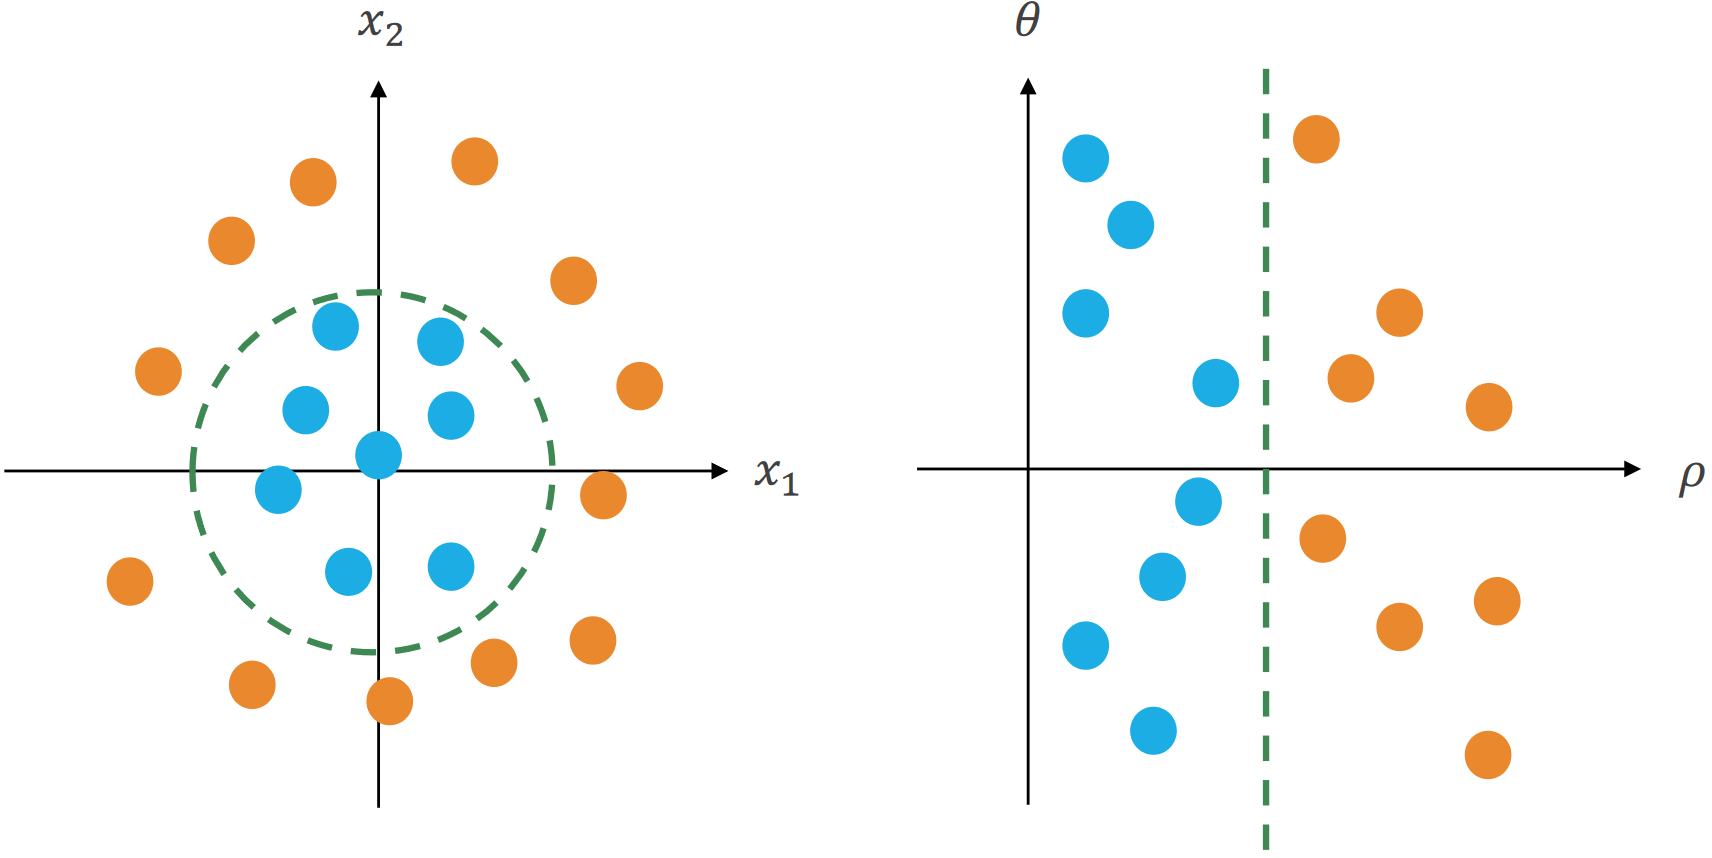
\includegraphics[width=0.40\linewidth]{./img/data_representation_linear.png}
        \caption{
            \parbox[t]{0.6\linewidth}{
                Example of non-linearly separable data points that become linearly separable in polar coordinates
            }
        }
    \end{figure}
\end{remark}



\section{Bag of visual words}

\begin{description}
    \item[Codeword] \marginnote{Codeword}
        Visual feature (e.g. an edge with a particular direction) that appears in an image.

    \item[Bag of visual words (BOVW)] \marginnote{Bag of visual words (BOVW)}
        Encoding of an image into a histogram of codeword frequencies.
\end{description}

\begin{figure}[H]
    \centering
    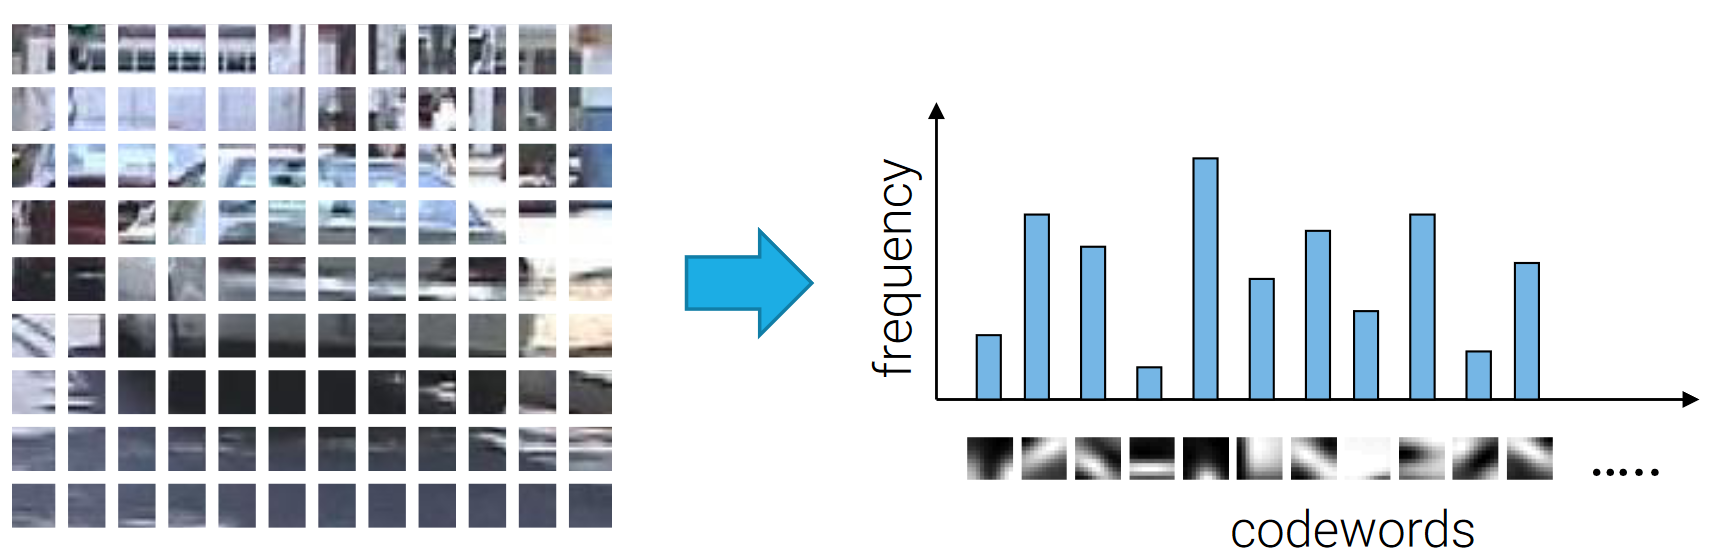
\includegraphics[width=0.6\linewidth]{./img/bovw.png}
\end{figure}



\section{Neural networks}

\begin{description}    
    \item[Shallow neural network] \marginnote{Shallow neural network}
        Linear transformations with an activation function:
        \[ 
            \begin{split}
                f(\vec{x}, \matr{\theta}) &= \matr{W}_2 \vec{h} + \vec{b}_2  \\
                &= \matr{W}_2 \phi(\matr{W}_1 \vec{x} + \vec{b}_1) + \vec{b}_2 = \vec{s}
            \end{split}
        \]
        where:
            \begin{itemize}
                \item $\matr{\theta} = (\matr{W}_1 \in \mathbb{R}^{h \times i}, \vec{b}_1 \in \mathbb{R}^{h}, \matr{W}_2 \in \mathbb{R}^{c \times h}, \vec{b}_2 \in \mathbb{R}^{c})$
                    are the parameters of the linear transformations with an inner representation of size $h$.
                \item $\phi$ is an activation function.
                \item $\vec{h}$ and $\vec{s}$ are activations.
            \end{itemize}

    \item[Activation function] \marginnote{Activation function}
        Function to introduce non-linearity.

        \begin{remark}
            Without an activation function, a neural network is equivalent to a plain linear transformation.
        \end{remark}

        Examples of activation functions are:
        \begin{descriptionlist}
            \item[Sigmoid] 
                Defined as:
                \[ 
                    \sigma(a) = \frac{1}{1+\exp(-a)} \hspace{2em}
                    \frac{\partial \sigma(a)}{\partial a} = \sigma(a) \big( 1-\sigma(a) \big)
                \]
                It is subject to the vanishing gradient problem.

            \item[Rectified linear unit (ReLU)] 
                Defined as:
                \[ 
                    \texttt{ReLU}(a) = \max\{ 0, a \} \hspace{2em}
                    \frac{\partial \texttt{ReLU}(a)}{\partial a} = \begin{cases}
                        1 & \text{if } a \geq 0\\
                        0 & \text{otherwise}
                    \end{cases}
                \]
                It is subject to the dead neuron problem for negative inputs.

            \item[Leaky ReLU] 
                Defined as:
                \[ 
                    \texttt{leaky\_ReLU}(a) = \begin{cases}
                        a & \text{if $a \geq 0$} \\
                        0.01 \cdot a & \text{otherwise}
                    \end{cases} \hspace{2em}
                    \frac{\partial \texttt{leaky\_ReLU}(a)}{\partial a} = \begin{cases}
                        1 & \text{if } a \geq 0 \\
                        0.01 & \text{otherwise}
                    \end{cases}
                \]
        \end{descriptionlist}

        \begin{example}[Linear separability]
            Linear transformations do not change the linear separability of the data points.
            A non-linear function can make linear separation possible.

            \begin{figure}[H]
                \centering
                \begin{subfigure}{0.6\linewidth}
                    \centering
                    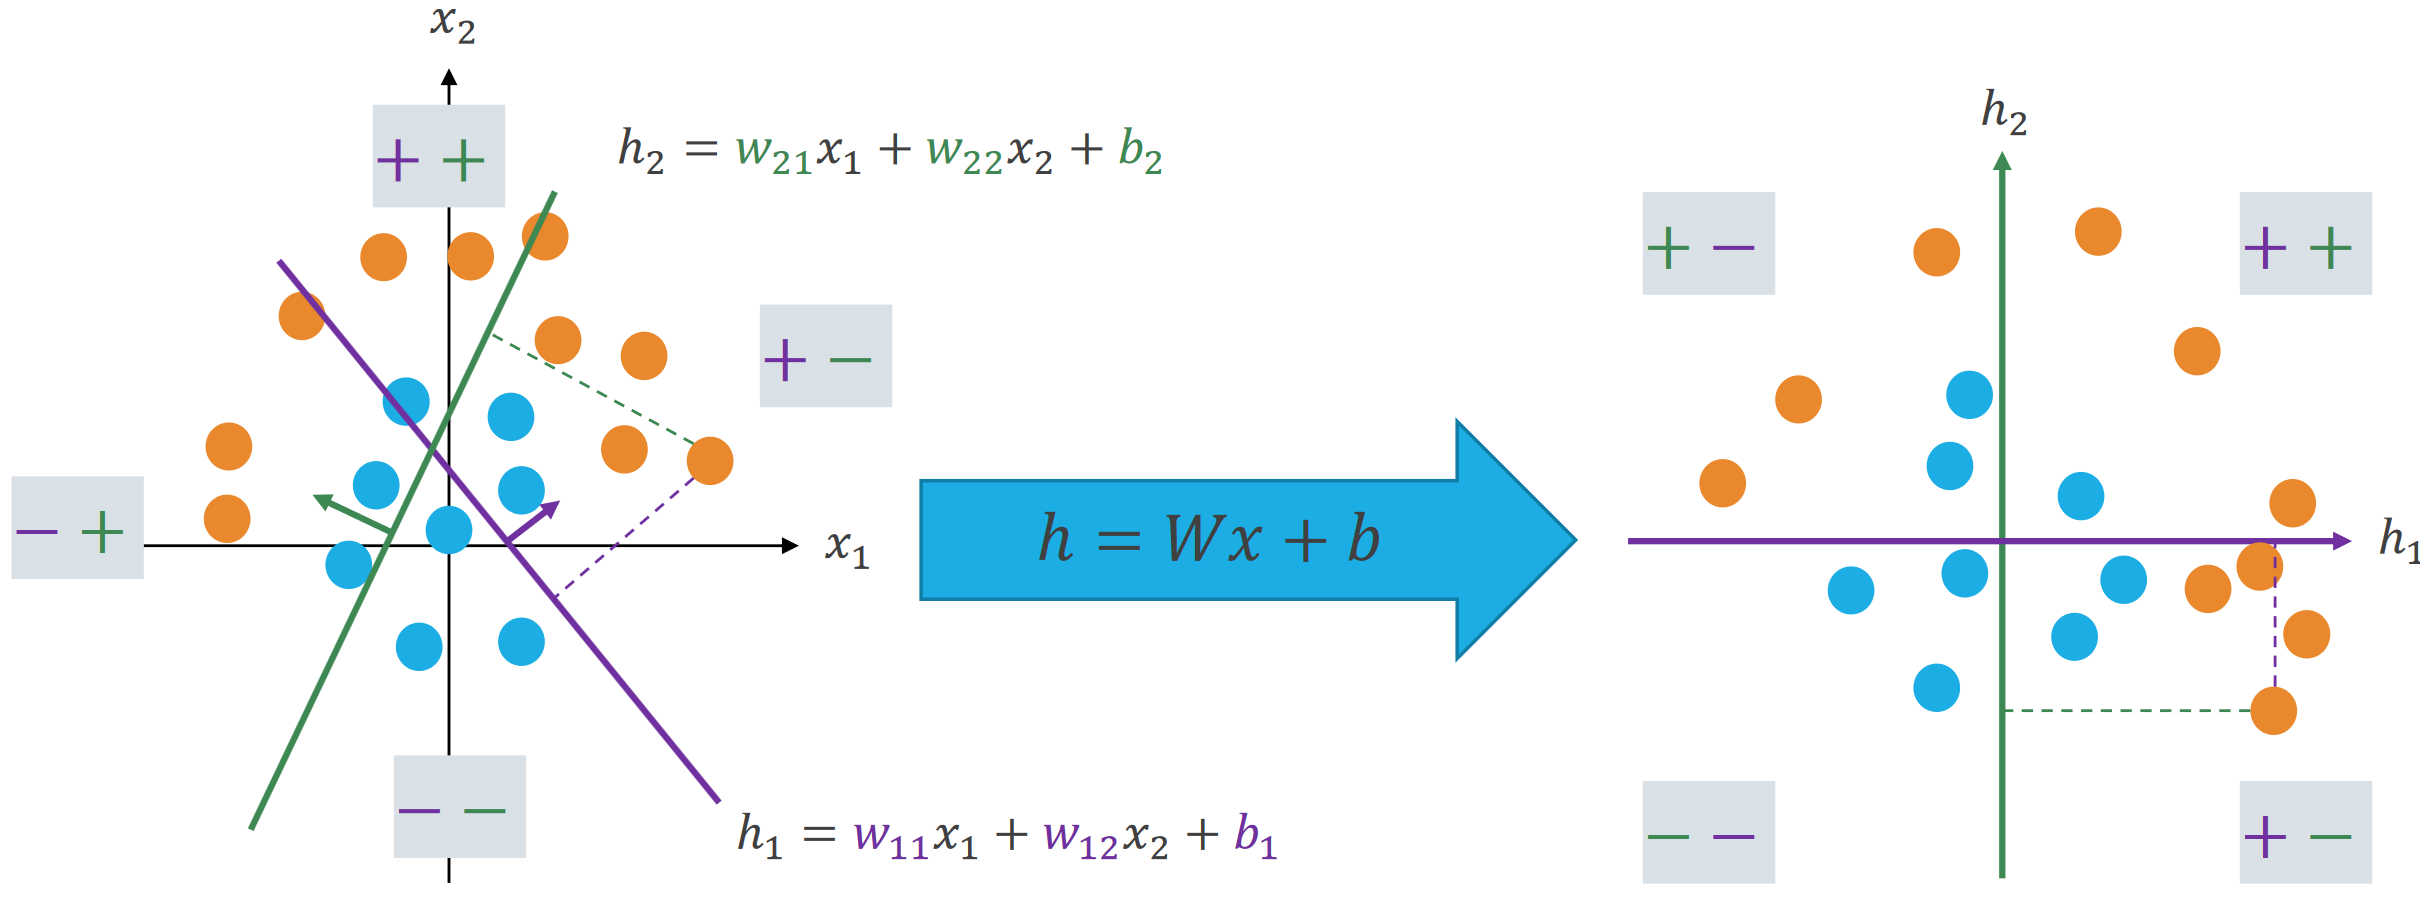
\includegraphics[width=\linewidth]{./img/relu_separability_1.png}
                \end{subfigure}

                \begin{subfigure}{0.6\linewidth}
                    \centering
                    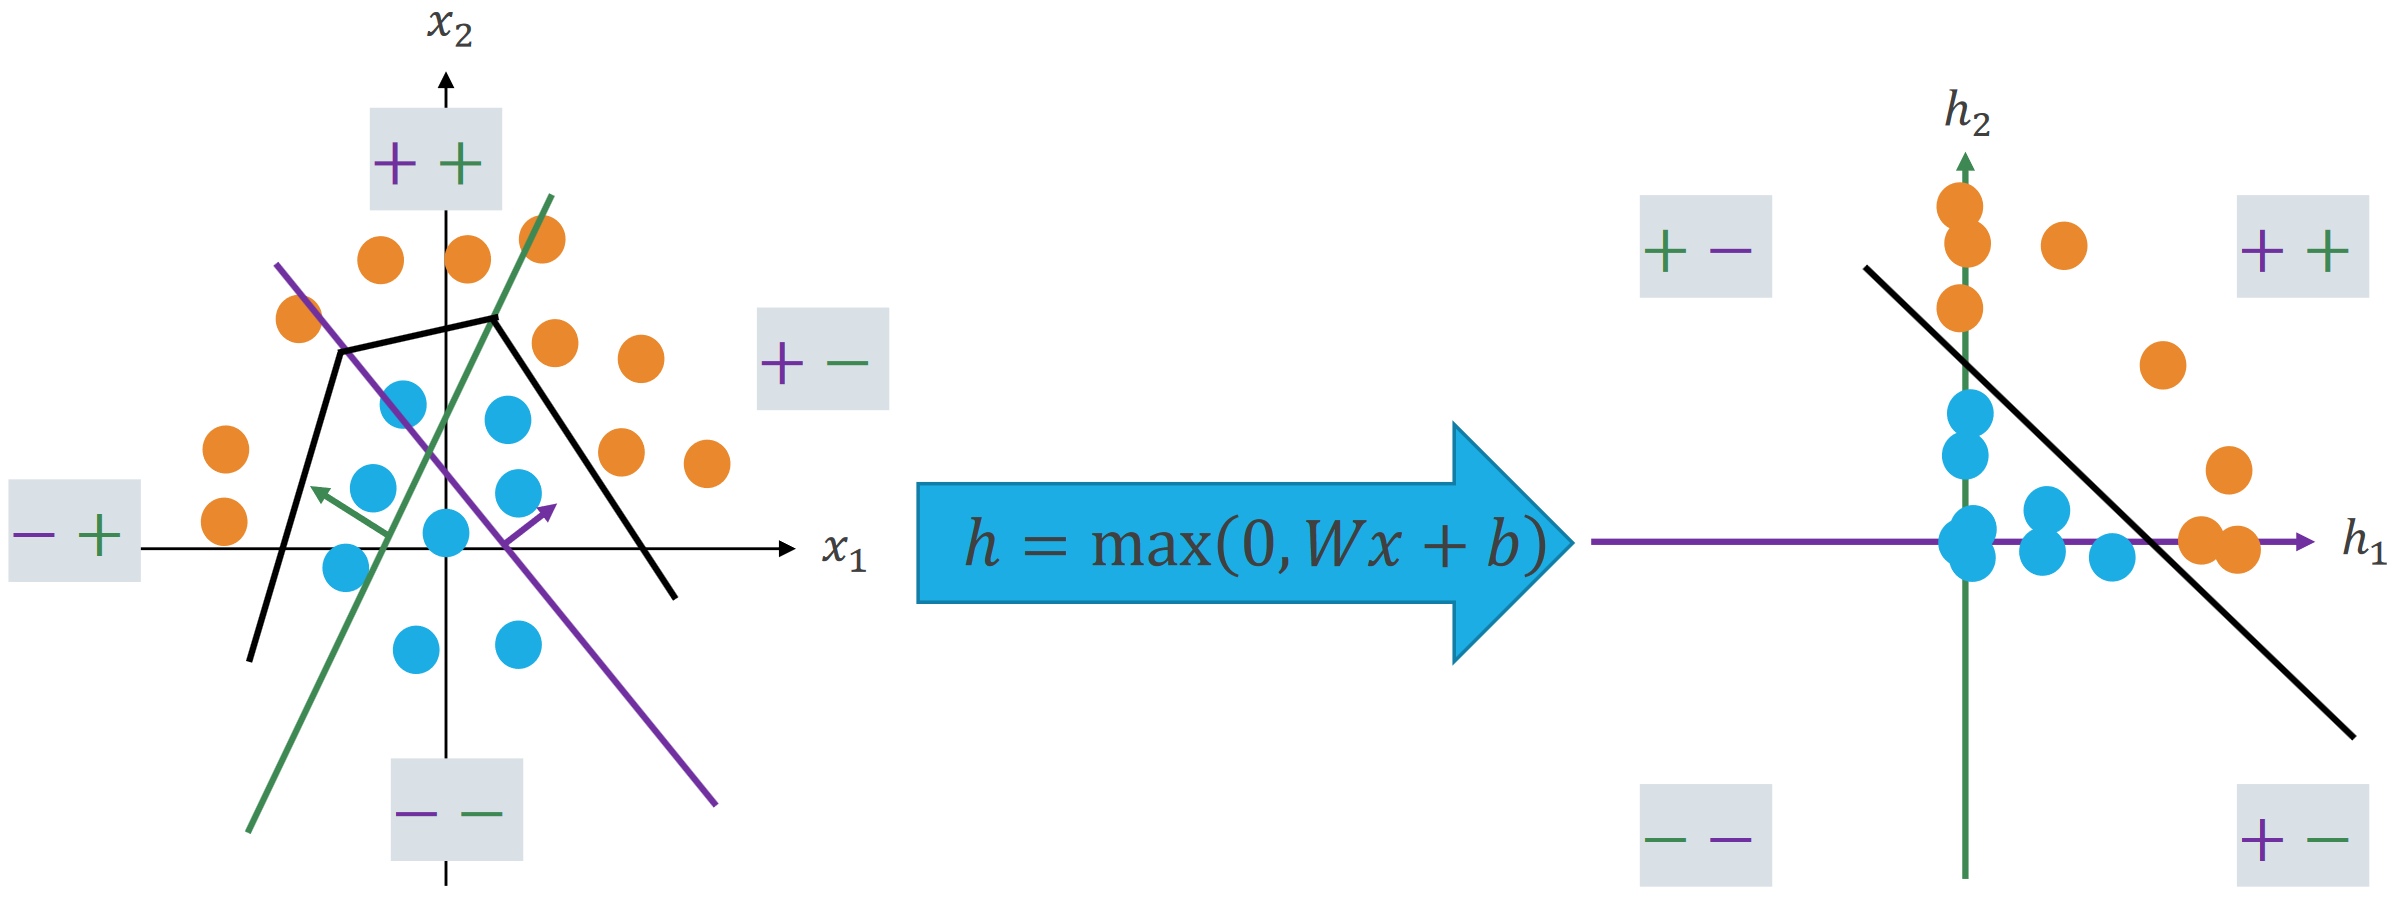
\includegraphics[width=\linewidth]{./img/relu_separability_2.png}
                \end{subfigure}
            \end{figure}
        \end{example}
    
    \item[Deep neural network] \marginnote{Deep neural network}
        Multiple layers of linear transformations and activation functions:
        \[
            \begin{split}
                f(\vec{x}, \matr{\theta}) &= \matr{W}_L \vec{h}_{L-1} + \vec{b}_L \\
                    &= \matr{W}_L \phi_L(\matr{W}_{L-1} \vec{h}_{L-2} + \vec{b}_{L-1}) + \vec{b}_L \\
                    &= \matr{W}_L \phi_{L}(\matr{W}_{L-1} \phi_{L-1}(\cdots \phi_{1}(\matr{W}_{1} \vec{x} + \vec{b}_{1}) \cdots) + \vec{b}_{L-1}) + \vec{b}_L = \vec{s} \\
            \end{split}  
        \]

        \begin{description}
            \item[Depth] Number of layers.
            \item[Width] Number of activations at each layer.  
        \end{description}
\end{description}



\section{Convolutional neural networks}


\subsection{Image filtering}

Consider the case of vertical edge detection.
Image filtering can be implemented through:
\begin{descriptionlist}
    \item[Fully-connected layer] \marginnote{Image filtering with fully-connected layers}
        Use an FC layer to transform the image.

        Given an image of size $H \times W$, the layer requires:
        \begin{itemize}
            \item $(H \cdot W) \cdot (H \cdot (W-1)) \approx H^2W^2$ parameters.
            \item $2 (H \cdot W) \cdot (H \cdot (W-1)) \approx 2H^2W^2$ FLOPs (multiplications and additions).
        \end{itemize}

    \item[Convolution/Correlation] \marginnote{Image filtering with convolutions}
        Use a convolution (more precisely, a cross-correlation) to transform the image.

        \begin{remark}
            Convolutions preserve the spatial structure of the image, have shared parameters and extract local features.
        \end{remark}

        Given an image of size $H \times W$, a convolution requires:
        \begin{itemize}
            \item $2$ parameters (in the case of edge detection).
            \item $3 (H \cdot (W-1)) \approx 3HW$ FLOPs.
        \end{itemize}

        \begin{description}
            \item[Convolution matrix] 
                A convolution can be expressed as a multiplication matrix such that:
                \begin{itemize}
                    \item The parameters are shared across rows.
                    \item The resulting matrix is sparse.
                    \item It adapts to varying input sizes.
                    \item It is equivariant to translation (but not w.r.t. rotation and scale).
                \end{itemize}

                \begin{figure}[H]
                    \centering
                    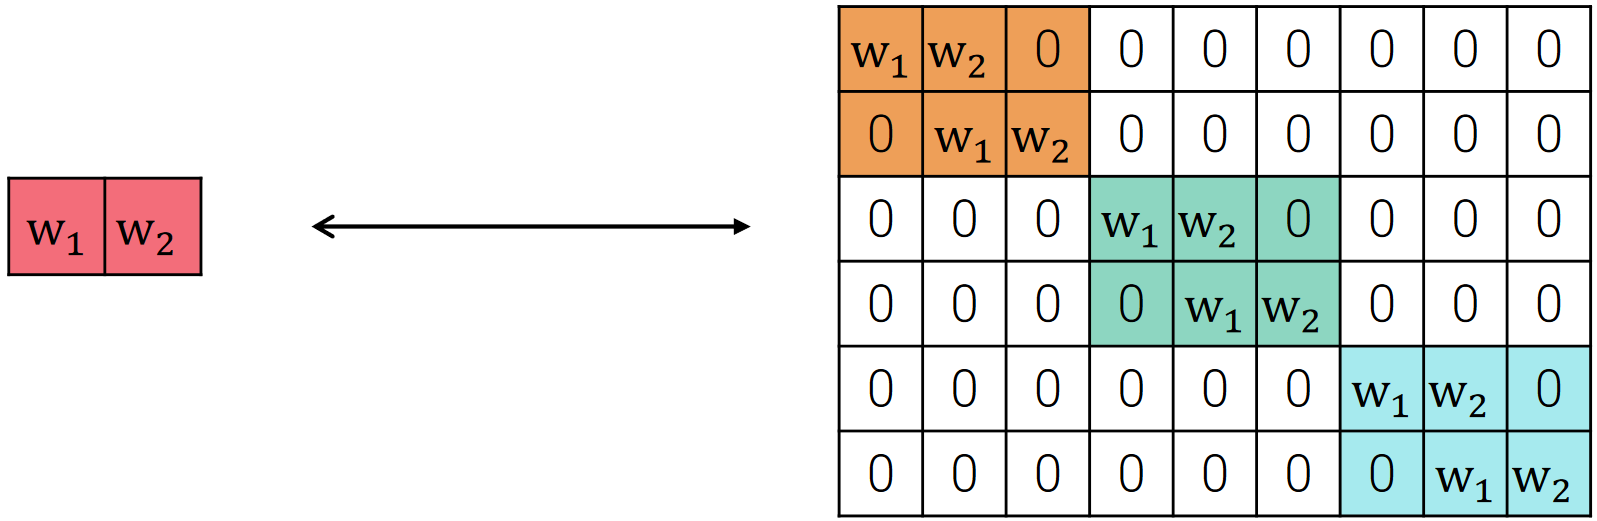
\includegraphics[width=0.45\linewidth]{./img/convolution_matrix.png}
                    \caption{Multiplication matrix of a $1 \times 2$ convolution}
                \end{figure}
        \end{description}
\end{descriptionlist}


\subsection{Convolutional layer} \label{sec:conv_layer}

\begin{description}
    \item[Multi-channel convolution] \marginnote{Multi-channel convolution}
        On inputs with multiple channels (e.g. RGB images), different 2D convolutions are applied across the different channels.

        Given a $C_\text{in} \times H_\text{in} \times W_\text{in}$ image $I$, a convolution kernel $K$ will have shape $C_\text{in} \times H_K \times W_K$
        and the output activation at each pixel is computed as:
        \[ 
            [K * I](j, i) = 
                \sum_{n=1}^{C_\text{in}} 
                \sum_{m = -\lfloor \frac{H_K}{2} \rfloor}^{\lfloor \frac{H_K}{2} \rfloor} 
                \sum_{l = -\lfloor \frac{W_K}{2} \rfloor}^{\lfloor \frac{W_K}{2} \rfloor} 
                    K_n(m, l) I_n(j-m, i-l) + b
        \]
        where $b$ is a bias term associated with the filter.

        \begin{figure}[H]
            \centering
            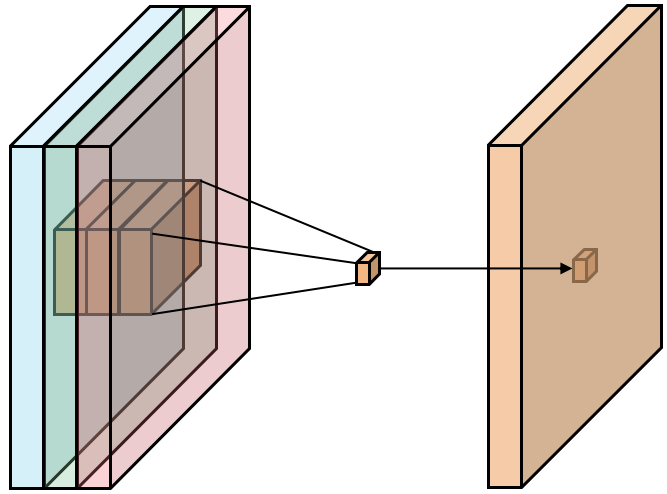
\includegraphics[width=0.2\linewidth]{./img/2d_convolution.png}
        \end{figure}

    \item[2D convolutional layer] \marginnote{2D convolutional layer}
        Given a $C_\text{in} \times H_\text{in} \times W_\text{in}$ image $I$ and a desired number of channels $C_\text{out}$ in the output activation,
        multiple different convolution kernels $K^{(i)}$ are applied and their results are stacked:
        \[
            [K * I]_k(j, i) = \sum_{n=1}^{C_\text{in}} \sum_{m} \sum_{l} K_n^{(k)}(m, l) I_n(j-m, i-l) + b^{(k)} \,\,\text{ for $k=1, \dots, C_\text{out}$} 
        \]

        \begin{figure}[H]
            \centering
            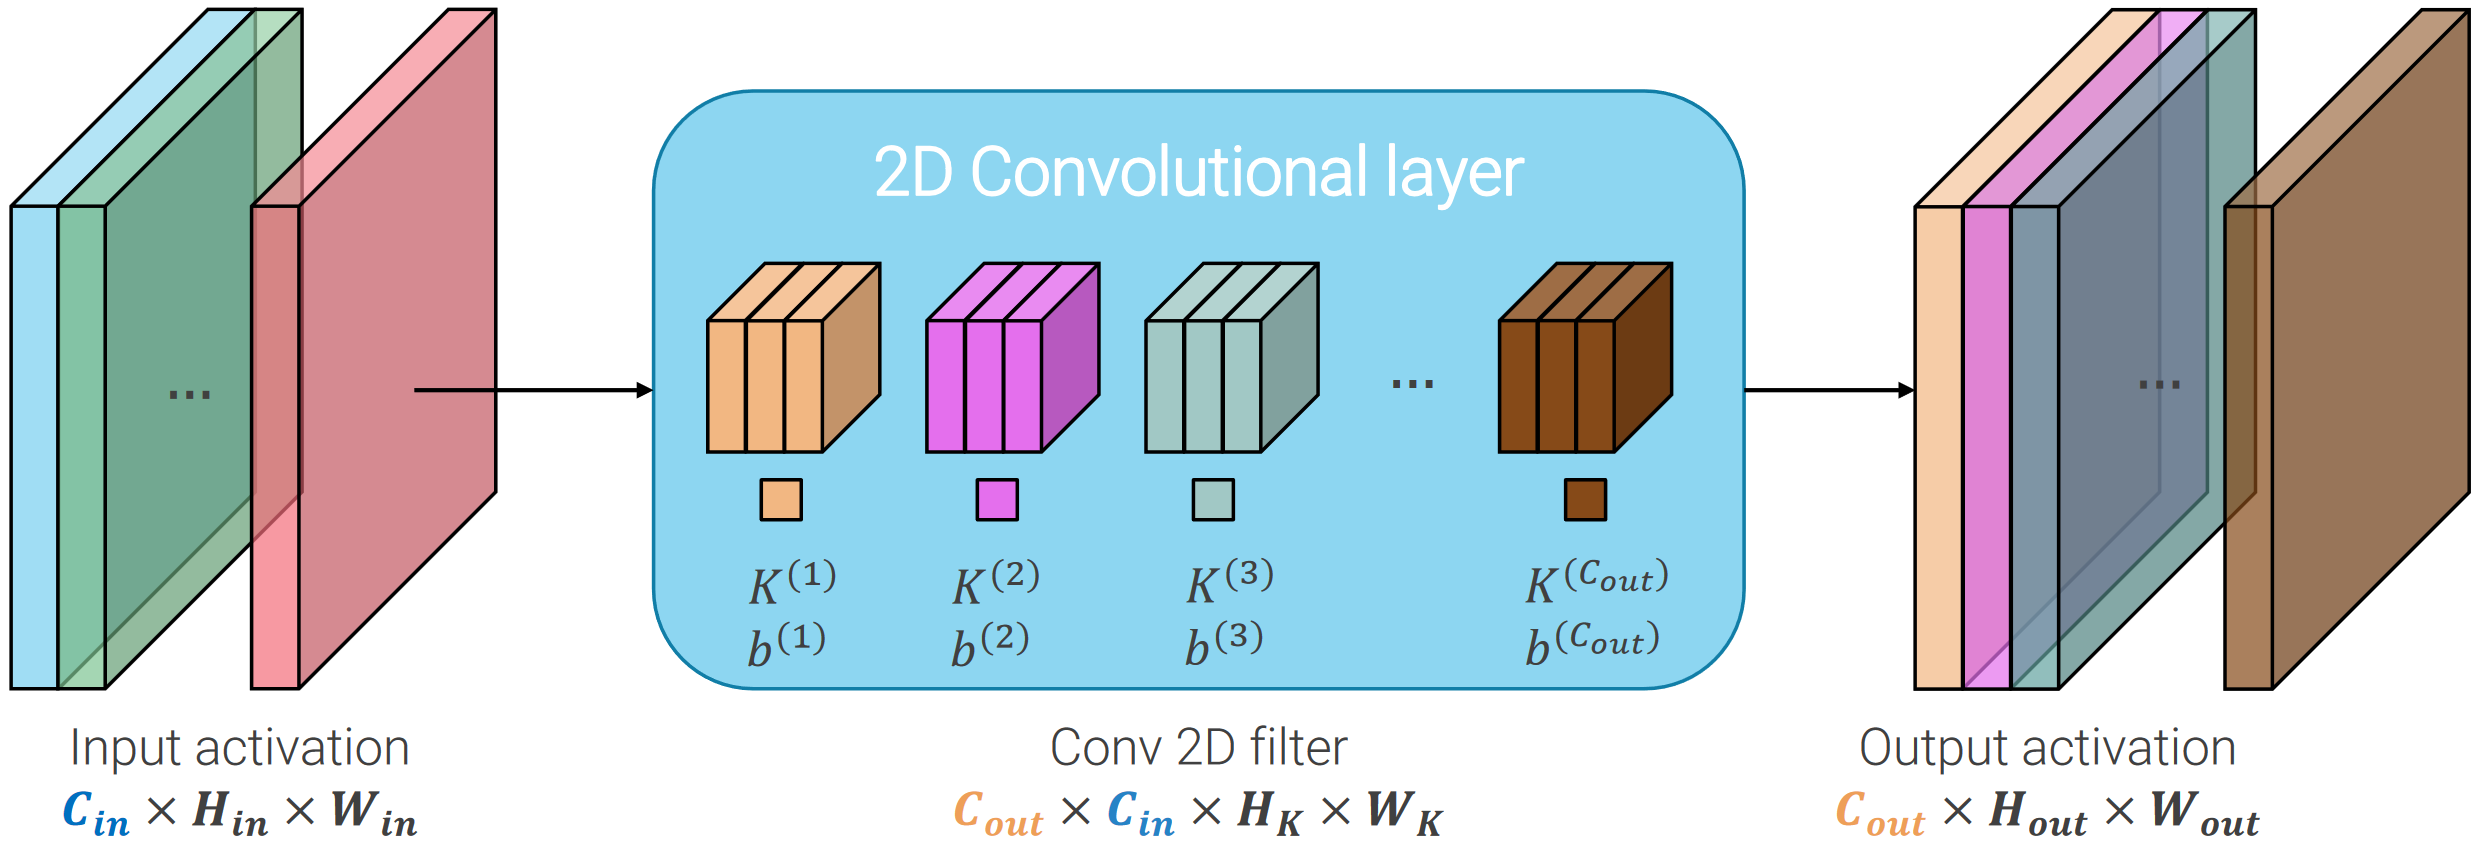
\includegraphics[width=0.65\linewidth]{./img/2d_convolution_multi_out.png}
        \end{figure}

        \begin{remark}
            Only applying convolutions results in a linear transformation of the input. Therefore, an activation function is applied after convolving.
        \end{remark}

    \item[Padding] 
        \phantom{}
        \begin{description}
            \item[No padding] \marginnote{No padding}
                Convolutions are only applied at pixels on which they do not overflow.

                Given a $H_\text{in} \times W_\text{in}$ image and a $H_K \times W_K$ kernel,
                the output shape is:
                \[ H_\text{out} = H_\text{in} - H_K + 1 \hspace{2em} W_\text{out} = W_\text{in} - W_K + 1 \]

                \begin{remark}
                    This type of padding is referred to as \texttt{valid}.
                \end{remark}

            \item[Zero padding] \marginnote{Zero padding}
                Zeros are added around the image.

                Given a $H_\text{in} \times W_\text{in}$ image and a $H_K \times W_K$ kernel,
                the padding is usually $P=\frac{H_K-1}{2}$ (for odd square kernels) and the output shape is:
                \[ H_\text{out} = H_\text{in} - H_K + 1 + 2P \hspace{2em} W_\text{out} = W_\text{in} - W_K + 1 + 2P \]

                \begin{remark}
                    This type of padding is referred to as \texttt{same}.
                \end{remark}
        \end{description}

        
    \item[Stride] \marginnote{Stride}
        Amount of pixels the convolution kernel is slid after each application. This is useful for downsampling the image.

        Given a $H_\text{in} \times W_\text{in}$ image and a $H_K \times W_K$ kernel,
        the output with stride $S$ and padding $P$ has shape:
        \[ 
            H_\text{out} = \left\lfloor \frac{H_\text{in} - H_K + 2P}{S} \right\rfloor + 1
            \hspace{2em} 
            W_\text{out} = \left\lfloor \frac{W_\text{in} - W_K + 2P}{S} \right\rfloor + 1
        \]
        
    
    \item[Receptive field] \marginnote{Receptive field}
        Number of pixels in the input image that affects a hidden unit.

        Given a $H_K \times W_K$ kernel, without stride, the receptive field of a neuron at the $L$-th layer is:
        \[ r_L = \big( 1 + L \cdot (H_K - 1) \big) \cdot \big( 1 + L \cdot (W_K - 1) \big) \]

        If each layer has a stride $S_l$, then the receptive field of the $L$-th activation is:
        \[ 
            r_L = \left( 1 + \sum_{l=1}^{L} \left( (H_K - 1) \prod_{i=1}^{l-1}S_i \right) \right) \cdot 
                \left( 1 + \sum_{l=1}^{L} \left( (W_K - 1) \prod_{i=1}^{l-1}S_i \right) \right)
        \]

        \begin{remark}
            Without stride, the receptive field grows linearly with the number of layers.
            With the same stride ($> 1$) across all the layers, the growth becomes exponential as $\prod_{i=1}^{l-1}S_i = S^{l-1}$.
        \end{remark}

    \item[Computational cost] \marginnote{Computational cost}
        \phantom{}
        \begin{description}
            \item[Parameters] 
                Given a $C_\text{in} \times H_\text{in} \times W_\text{in}$ image, a kernel $H_K \times W_K$ and a desired number of output channels $C_\text{out}$,
                the corresponding convolutional layer has the following number of parameters:
                \[ C_\text{out} ( C_\text{in} H_K W_K + 1 ) \]

            \item[Floating-point operations] 
                Given a $C_\text{in} \times H_\text{in} \times W_\text{in}$ input image, a kernel $H_K \times W_K$ and 
                the corresponding output image of size $C_\text{out} \times H_\text{out} \times W_\text{out}$,
                the number of FLOPs (multiplications and additions) is:
                \[ 2 (C_\text{out} H_\text{out} W_\text{out}) (C_\text{in} H_K W_K) \]

            \item[Multiply-accumulate operations] 
                A MAC operation implemented in hardware allows to perform a multiplication and an addition in a single clock cycle.
                Therefore, the number of MACs is:
                \[ \cancel{2} (C_\text{out} H_\text{out} W_\text{out}) (C_\text{in} H_K W_K) \]
        \end{description}
    
    \item[Other convolutional layers]
        \phantom{}
        \begin{description}
            \item[1D convolutional layer] \marginnote{1D convolutional layer}
                Suitable for time series.
                \[
                    [K * S]_k(i) = \sum_{n=1}^{C_\text{in}} \sum_{l} K_n^{(k)}(l) S_n(i-l) + b^{(k)}
                \]

            \item[3D convolutional layer] \marginnote{3D convolutional layer}
                Suitable for videos.
                \[
                    [K * V]_k(h, j, i) = \sum_{n=1}^{C_\text{in}} \sum_{p} \sum_{m} \sum_{l} K_n^{(k)}(p, m, l) V_n(h-p, j-m, i-l) + b^{(k)}
                \]
        \end{description}
\end{description}


\subsection{Pooling layer}
\marginnote{Pooling layer}

Kernel that aggregates several values through a fixed function into one output.
Each input channel is processed independently (i.e. $C_\text{in} = C_\text{out}$).

\begin{remark}
    Traditionally, pooling layers were used for downsampling. Therefore, the stride is usually $> 1$.
\end{remark}

\begin{description}
    \item[Max pooling] \marginnote{Max pooling}
        Select the maximum within the kernel.

        \begin{remark}
            Max pooling is invariant to small (depending on the receptive field, it can also be big w.r.t the input image) spatial translations.
        \end{remark}
\end{description}

\begin{remark}
    Mean pooling can be represented through normal convolutions.
\end{remark}


\subsection{Batch normalization layer}
\marginnote{Batch normalization layer}

Normalize the output of a layer during training in such a way that it has zero mean and unit variance.

\begin{description}
    \item[Training]
        During training, normalization is done on the current batch.
        Given the $B$ activations of a batch $\{ \vec{a}^{(i)} \in \mathbb{R}^{D} \mid i = 1, \dots, B \}$, 
        mean and variance are computed as:
        \[ 
            \vec{\mu}_j = \frac{1}{B} \sum_{i=1}^{B} \vec{a}_j^{(i)} 
            \hspace{1.5em} 
            \vec{v}_j = \frac{1}{B} \sum_{i=1}^{B} \left( \vec{a}_j^{(i)} - \vec{\mu}_j \right)^2 
            \hspace{2em}
            \text{ for $j = 1, \dots, D$} 
        \]

        Then, the normalized activation is computed as:
        \[ \hat{\vec{a}}_j^{(i)} = \frac{\vec{a}_j^{(i)} - \vec{\mu}_j}{\sqrt{\vec{v}_j + \varepsilon}} \hspace{2em} \text{ for $j = 1, \dots, D$} \]
        where $\varepsilon$ is a small constant.

        To introduce some flexibility, the final activation $\vec{s}^{(i)}$ is learned as:
        \[ \vec{s}_j^{(i)} = \vec{\gamma}_j \hat{\vec{a}}_j^{(i)} + \vec{\beta}_j \hspace{2em} \text{ for $j = 1, \dots, D$} \]
        where $\vec{\gamma}_j$ and $\vec{\beta}_j$ are parameters.

        To estimate the mean and variance of the entire dataset to use during inference, their running averages are also computed.
        At the $t$-th step, the running averages of mean and variance are computed as:
        \[ 
            \vec{\mu}_j^{(t)} = (1-\beta) \vec{\mu}_j^{(t-1)} + \beta \vec{\mu}_j 
            \hspace{1.5em} 
            \vec{v}_j^{(t)} = (1-\beta) \vec{v}_j^{(t-1)} + \beta \vec{v}_j 
            \hspace{2em} \text{ for $j = 1, \dots, D$} 
        \]
        where $\beta$ is the momentum (usually $\beta = 0.1$).

        \begin{remark}
            All training steps of batch normalization are differentiable and can be integrated into gradient descent.
            If normalization is done outside gradient descent, the optimization process might undo it.
        \end{remark}

        \begin{remark}
            For convolutional layers, mean and variance are computed along the spatial dimension (i.e. pixels in the same output channel are normalized in the same way).
        \end{remark}


    \item[Inference] 
        During inference, the final running averages of mean $\vec{\mu}$ and variance $\vec{v}$ are used to normalize the activations (i.e. they are considered constants).
        Given the learned parameters $\vec{\gamma}$ and $\vec{\beta}$, an activation is normalized as follows:
        \[  
            \begin{split}
                \vec{s}_j^{(i)} &= \vec{\gamma}_j \frac{\vec{a}_j^{(i)} - \vec{\mu}_j}{\sqrt{\vec{v}_j + \varepsilon}} + \vec{\beta}_j \\
                &= \left( \frac{\vec{\gamma}_j}{\sqrt{\vec{v}_j + \varepsilon}} \right) \vec{a}_j^{(i)} + 
                    \left( \vec{\beta}_j - \frac{\vec{\gamma}_j \vec{\mu}_j}{\sqrt{\vec{v}_j + \varepsilon}} \right)
            \end{split}
            \hspace{2em} \text{ for $j = 1, \dots, D$} 
        \]
        
        \begin{remark}
            Normalization during inference can be seen as a linear transformation. Therefore, it can be merged with the previous layer.
        \end{remark}


    \item[Properties]
        The advantages of batch normalization are:
        \begin{itemize}
            \item It allows to use a higher learning rate and makes initialization less important.
            \item Training becomes non-deterministic (i.e. adds noise) acting as some form of regularization.
            \item During inference, there is no overhead as it can be merged with the previous layer.
        \end{itemize}
        The disadvantages are:
        \begin{itemize}
            \item It is not clear why it works.
            \item Training and inference work differently.
            \item It does not scale with batches that are too small.
        \end{itemize}

        \begin{remark}[Internal covariate shift]
            A possible motivation for batch normalization is that each layer of a neural network expects an input distribution that changes at each training iteration.
            On the other hand, the distribution of the input itself depends on the previous layer and it also changes at each iteration.
            Therefore, each layer is disrupted by the update of the previous one. Batch normalization aims to minimize this by maintaining a fixed distribution.
        \end{remark}
\end{description}